\documentclass[11pt]{scrreprt}
\usepackage[utf8]{inputenc}
\usepackage{graphicx}
\usepackage[hidelinks]{hyperref}
\usepackage{listings}
\usepackage{longtable}
\usepackage{multicol}
\usepackage{booktabs} % http://ctan.org/pkg/booktabs
\usepackage[numbib,notlof,notlot,nottoc]{tocbibind} % % http://www.ctan.org/pkg/tocbibind

\makeatletter
\renewenvironment{thebibliography}[1]
     {\section{\bibname}% <-- this line was changed from \chapter* to \section
      \@mkboth{\MakeUppercase\bibname}{\MakeUppercase\bibname}%
      \list{\@biblabel{\@arabic\c@enumiv}}%
           {\settowidth\labelwidth{\@biblabel{#1}}%
            \leftmargin\labelwidth
            \advance\leftmargin\labelsep
            \@openbib@code
            \usecounter{enumiv}%
            \let\p@enumiv\@empty
            \renewcommand\theenumiv{\@arabic\c@enumiv}}%
      \sloppy
      \clubpenalty4000
      \@clubpenalty \clubpenalty
      \widowpenalty4000%
      \sfcode`\.\@m}
     {\def\@noitemerr
       {\@latex@warning{Empty `thebibliography' environment}}%
      \endlist}
\makeatother


\newcommand{\tabitem}{~~\llap{\textbullet}~~}
\newcommand*{\SignAndDate}[1]{%
    \par\noindent\makebox[2.5in]{\hrulefill} \hfill\makebox[2.0in]{\hrulefill}%
    \par\noindent\makebox[2.5in][l]{#1}      \hfill\makebox[2.0in][l]{Date}%
}%

\title{\textbf{Clang AST Analysis and Repair}}
\subtitle{2014-2015 Computer Science Capstone Project}
\author{Nicholas Nelson\\
		Charles Santos}
\date{}
\begin{document}

\maketitle

\tableofcontents

\chapter{Project Introduction}

This project was requested by Garmin AT Inc., a subsidiary of Garmin Corporation, as part of their ongoing commitment to engineering education at Oregon State University and the continued growth of software engineering requirements within their internal software development teams.

Garmin AT focuses on avionics and navigational electronics for use within private and commercial aircraft.
This equipment contains embedded firmware and software written in C and requiring exacting standards and precision under Federal Aviation Administration (FAA) guidelines prior 
to use in production products.
Combining these FFA standards with Garmin AT's internal style and formatting guidelines has meant that evaluating and fixing compliance issues has been a time consuming process.

The purpose of this project was to use an internally developed code review tool as a baseline to develop a modular application that leverages the LLVM project's Clang AST interpreter libraries\footnote{http://clang.llvm.org/} and the Python regular expression libraries to process rulesets for each style and formatting requirement.

The project team consisted of Andrew Stucky, Embedded Software Engineer at Garmin AT, Nicholas Nelson and Charles Santos, both of whom are senior Computer Science students at Oregon State University.
As the project sponsor and mentor, Andrew provided the project requirements, initial codebase, and testing infrastructure.
Nick Santana, a member of Andrew's development team, provided support for the runtime codebase and assisted with the integration of changes to the infrastructure that runs the rulesets.

The entire project codebase was maintained using \texttt{git} version control on GitHub\footnote{https://github.com/}, and utilized the project management capabilities of that platform.
The project was designed in a modular fashion to allow individual formatting rules to be developed and tracked in separate branches.
Issues for each rule, submitted by Andrew, were used to document requirements, design decisions, team communications, and status updates.
Pull requests between development branches and the master branch were used to alert Andrew that a potential solution to a specific rule was ready for final testing and integration into the codebase that would be included in one of three major version releases that occurred during the project.

\chapter{Original Client Requirements Document} \label{orig_req_doc}

\section{Project Demographics}

\renewcommand{\arraystretch}{1.2}
\noindent\begin{tabular}{p{3cm}p{8cm}}
Project Name:   & \begin{tabular}[t]{l}CASTAR: Clang AST Analysis \& Repair\end{tabular}\\
Team Name:      & \begin{tabular}[t]{l}Team \#45 - Lúdramán Industries\end{tabular}\\
Team Members:   & \begin{tabular}[t]{l}Nicholas Nelson\\ Mark Mills\\ Charles Santos\end{tabular}\\
Client/Sponsor: & \begin{tabular}[t]{l}Andrew Stucky, Garmin AT\\\textit{andrew.stucky@garmin.com}\end{tabular}
\end{tabular}

\section{Introduction}
Garmin AT develops navigational components for a variety of aircraft. These components provide a high degree of situational awareness to pilots by integrating data from a variety of sources including GPS, weather, and traffic information from the Automatic Dependent Surveillance-Broadcast (ADS-B) data link network. Avionics displays similar to the products Garmin produces were crucial to the Capstone Program in Alaska which reduced accidents state wide by 40\% from 1999 to 2009 according to a report published by the Federal Aviation Administration.

Avionics software must meet Federal Aviation Administration (FAA) guidelines for safety and operations certification, specifically DO-178B/ED-12B (Software Considerations in Airborne Systems and Equipment Certification), prior to being allowed within any operational aircraft.

Garmin AT currently utilizes Python regular expression scripts for internally evaluating code quality and standards prior to submitting for FAA certification. We have been tasked with reimplementing and expanding functionality to take advantange of the Clang AST parser library. These changes will allow more complex rulesets that can flag potential syntax irregularities and automatically correct them if possible; or allowing for human review otherwise.

\section{Project Description}
Garmin’s avionics products are powered by embedded firmware and software written in C. There are serious safety considerations for any code embedded in avionics components; a bug at the wrong time could result in serious injury or death to the pilot and passengers of the craft relying on this software. Therefore embedded avionics software must follow precise quality control guidelines established by the FAA. Garmin also has internal style and formatting guidelines that they would like to enforce. Garmin has automated some quality control for these guidelines using regular expressions. However regular expressions are difficult to maintain and many of the rules are not easily implemented using regular expressions. Now Garmin is looking to implement these rules using python scripts and to create scripts for many of the rules that have not yet been implemented using regular expressions.

Our scripts will be examining abstract syntax trees to determine if the source code is compliant with FAA and Garmin guidelines. We will be using abstract syntax trees provided by Clang to examine C source code using python scripts. When a script finds a violation of the guidelines it will either make the necessary change or alert the user to the problem.

The client has provided us with the list of rules/issues that need to be implemented in python in rule specific scripts. There may be a number of issues that are more appropriate as regular expressions and that will have to be determined as we progress and consult with the client. Some of these python scripts may group together multiple issues that are related. Users will specify C source/header files that need to be checked, our main script will use Clang to parse the abstract syntax trees from these files. The main script will then call scripts for each of the rule specific scripts which will examine the ASTs for compliance with the issues the client has identified. When there is a violation there will either be a change to the source or a flag will be logged to alert the user. The scripts which are allowed to change source code will be run first followed by scripts that can only alert the user since it is possible that some changes may mitigate these warnings. We will also need to determine an order of operations for any scripts that change source code since they may interact with one another in ways that may either create new issues or resolve errors before they are handled by later scripts. If the source code is changed Clang will be called again and the altered AST will be loaded.

\section{Requirements}
The following list constitutes the baseline of requirements that will completed during this project. We will switch issues from this list and the Issues list (Section~\ref{issues}) as needed based upon the priorities of the client/mentor, and the applicability of an issue to being resolved using the Clang AST library. Issues not on the Requirements list will still be attempted and hopefully completed during this project.

\begin{longtable}{| p{.30\textwidth} | p{.65\textwidth} |} 
\hline
\textbf{Requirement} & \textbf{Description}\\ \hline
Inline Comments & This method will wrap inline comments on words and begin/end them at the user specified column numbers.\\ \hline
In-function Comments & This method will align all block comments within functions to the line below the comment. They will end on the user specified value.\\ \hline
Title Header Comments & This method will find title heading comments outside of functions and align them to the user specfied value. The heading itself will be capitalized and centered within the block.\\ \hline
Public/Private Trimming & This method will trim out the public/private functions from the file header comment block, if they are present.\\ \hline
Hard Tabs & Hard tabs need to be converted to four-space tabs in order to circumvent short-tabbing anything.\\ \hline
Slash Slash Comments & This method will search out double slash comments and, if specified by the user, delete them. Otherwise, the user will be warned of their presence, which should not be present within production code.\\ \hline
File Header Comment & This method will search through each file header comment block and function header comment block and find the little addendum after the function name /file name/dash and trim that section out.\\ \hline
\texttt{NoKeywords} & This method will remove the "NoKeywords" keyword in the file header comment block.\\ \hline
Copyright Format & This method will force the copyright year string within the file header comment block to match the XYZ example along with setting it to the correct year.\\ \hline
Stack Function Arguments & This method will stack function arguments within each parameter list in the source file.\\ \hline
Brace alignment & This method will align braces with a tab for each previous active brace.\\ \hline
Parentheses Whitespace & This method will make all code items within parentheses look like ``( this )''. Comments are unaffected by this rule.\\ \hline
Local Variables Section & This method will move local variables to the top of their enclosing function and mark them with a comment block.\\ \hline
Includes formatting & This method will group includes into an ANSI group, a GRM group, a public group, and a private group. It will then place a space between each group, case them down, and write them to the top of the file.\\ \hline
Prototype Static Functions & This method will prototype functions that are not already prototyped but are static at the top of the file. They will be sorted and spaced correctly, and have the static qualifier added to the prototype and function as appropriate.\\ \hline
File Assertion & This method will match the file assertion at the top of the file to the actual source file name. If the file name is present along with "assert" in the same line, it is assumed that the file assertion is correct and present.\\ \hline
Line Endings & This method will enforce line endings as newline/carriage returns. This is automatically done whenever any issue is run.\\ \hline
In-line comment upgrade & This method will upgrade inline comments on their own line into block comments.\\ \hline
Function Order & This method will reorganize functions into alphabetical order with public first, then private, then local.\\ \hline
Invalid private includes for component & This method will validate that private includes are appropriate for the component.\\ \hline
Missing Sections & This method will validate that all required sections (i.e. General Includes, Types, etc.) exist in the file.\\ \hline
\texttt{Void} Functions & This method will validate that any function prototypes with no arguments will use the \texttt{void} parameter modifier.\\ \hline
End of Function Comments & This method will validate that all functions contain a ``end of function'' comment.\\ \hline
Typedef Comments & This method will validate that all \texttt{typedef} declarations include an accompanying comment.\\ \hline

\end{longtable}

\section{Versions}

Our version control model will consist of several branches, both permanent and temporary, which will allow us to have sane coding practices and reduce merge conflicts by grouping feature development, bugfixes, testing, release staging, and production releases into separate branches. See Figure~\ref{fig:versioning} for an illustration of our model.

Our version numbering scheme will consist of a \textit{M.n} format, where \textit{M} is a major release and \textit{n} is a minor release (i.e. 2.7 to 2.8 would be a minor release, 2.8 to 3.0 would be a major release).

Our major version release schedule will be the following:
\begin{itemize}
	\item \textbf{Version 1.0} released on December 8, 2014
	\subitem 8-10 issues resolved through completed rule methods
	\item \textbf{Version 2.0} released on March 13, 2015
	\subitem 10-14 issues resolved through completed rule methods
	\item \textbf{Version 3.0} released on May 8, 2015
	\subitem 6-10 issues resolved through completed rule methods
\end{itemize}

These major version releases are timed to coincide with the end of the Fall, Winter, and Spring terms to allow for concise divisions of labor and evaluation for our team. Spring term is shifted in order to meet the deadline for presentation at the EXPO event.

Minor version releases will occur based upon the completion of development, testing, and quality assurance of issues. The client/mentor has final approval of all releases, and can dictate when issues require additional development and testing prior to release.

\begin{figure}[hp]
  \caption{Version Control Model}
  \makebox[\textwidth][c]{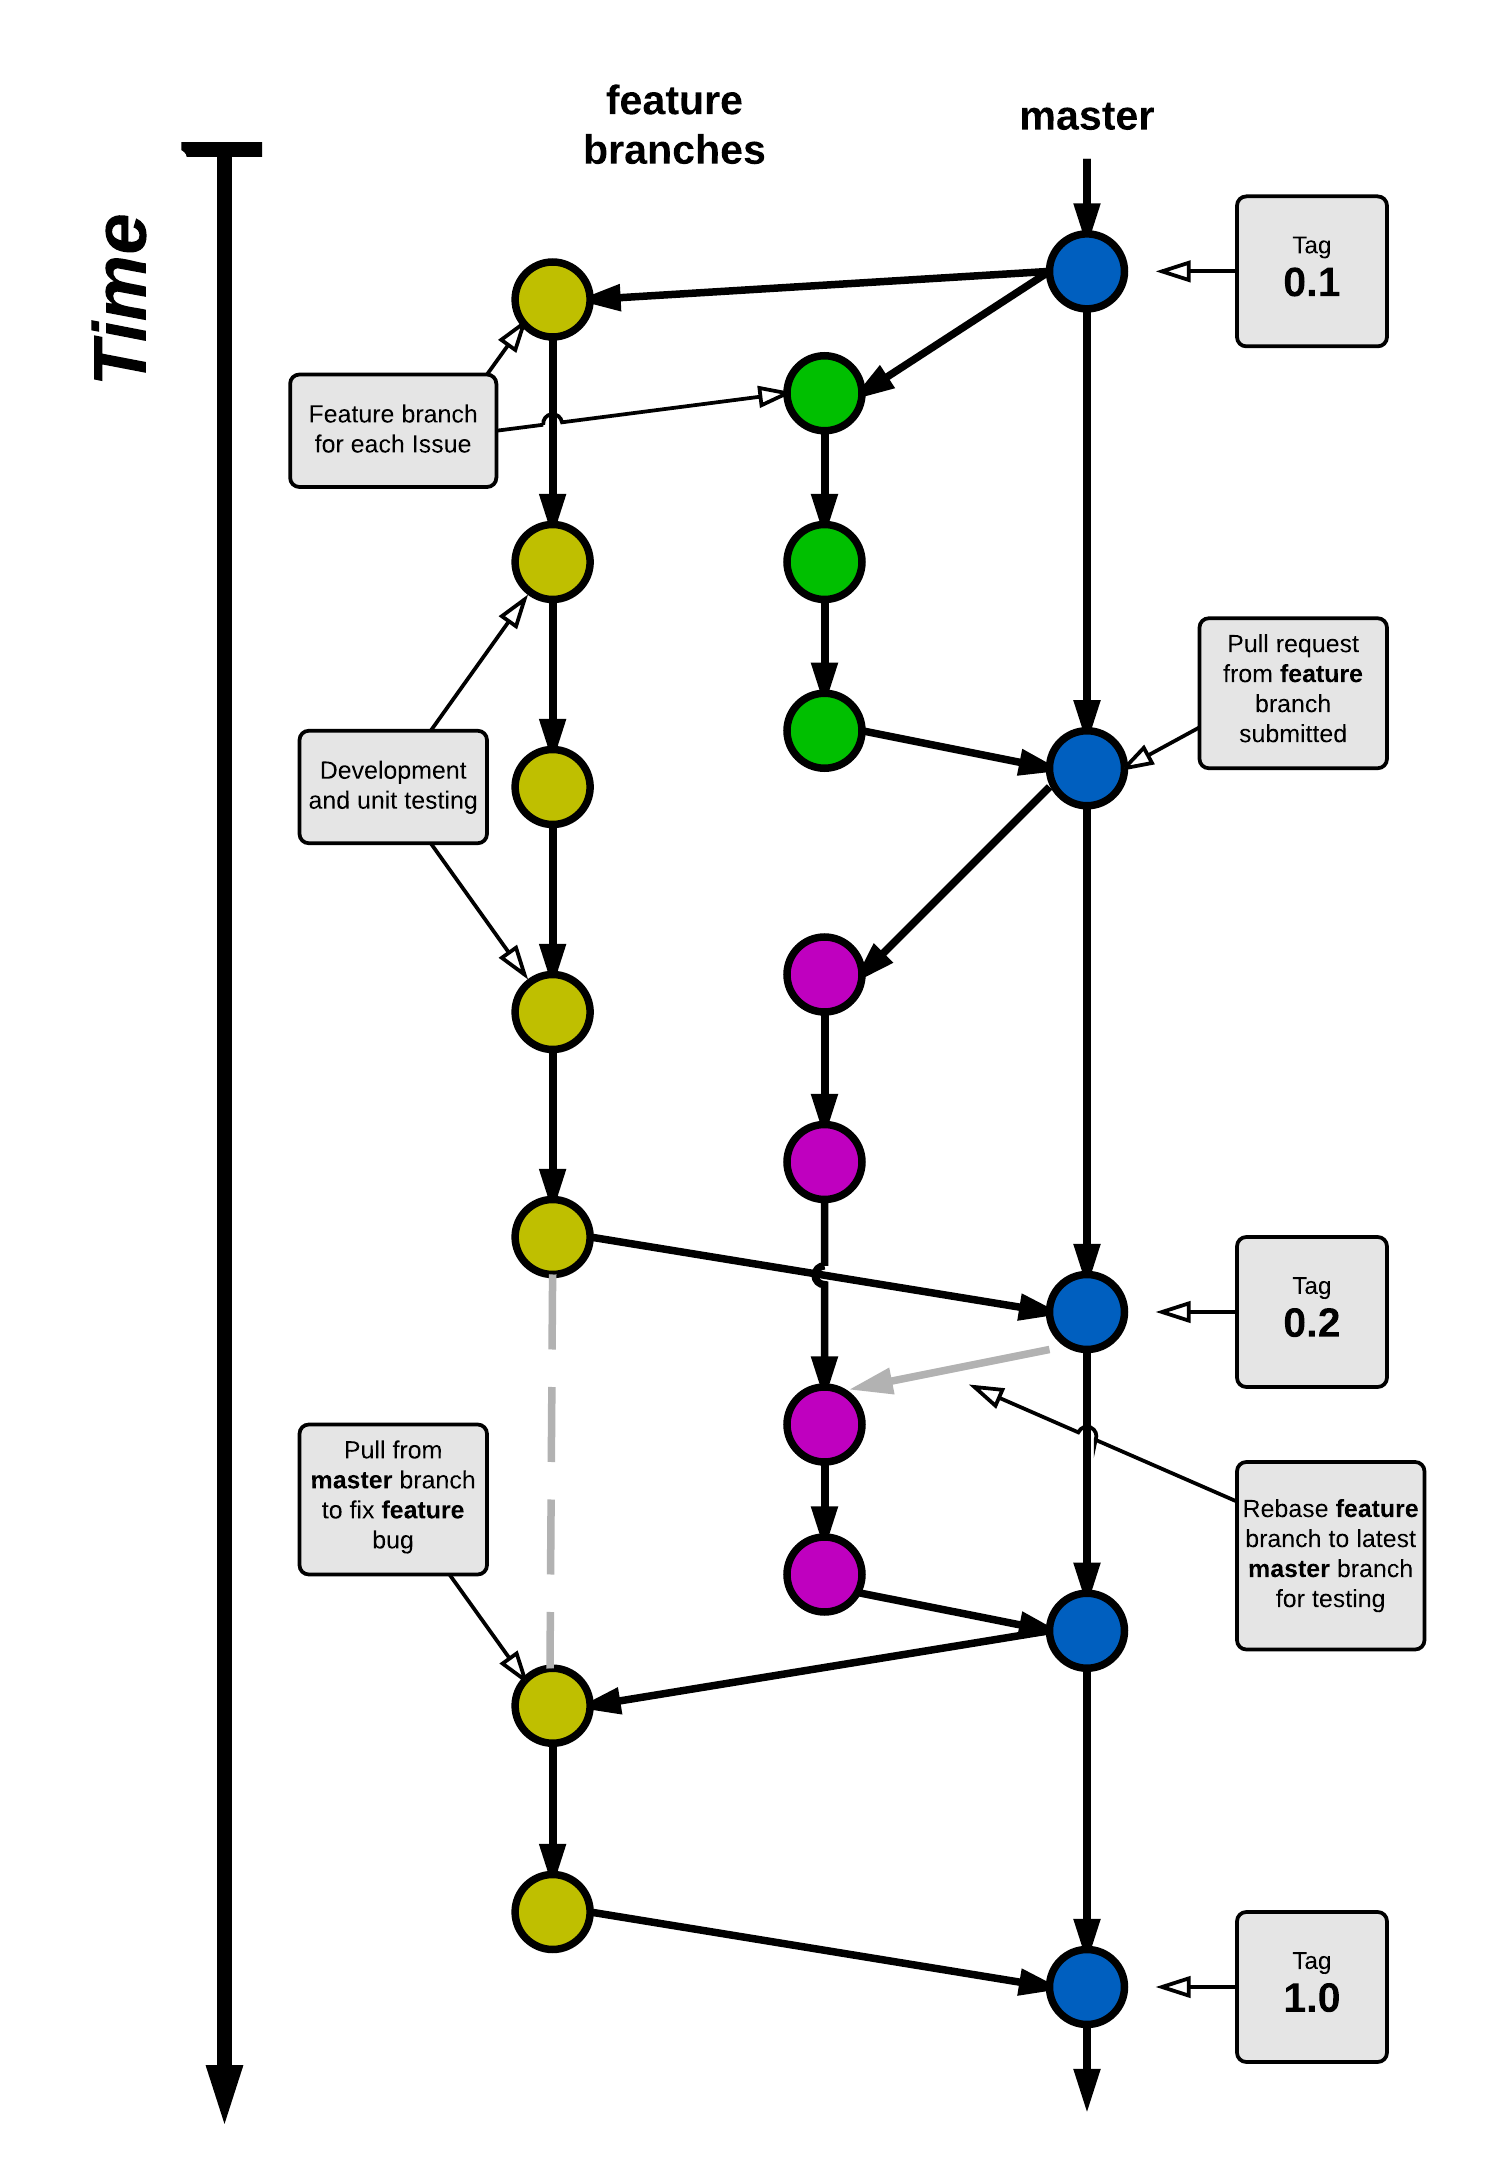
\includegraphics[width=1.0\textwidth]{version_control_model}}%
  \label{fig:versioning}
\end{figure}

\section{Design}
Fundamentally, our project and the design to complete it relies upon Abstract Syntax Tree (AST) representations of C source code and the methods in which the Clang AST parser library represents those AST trees. Therefore we have relied heavily upon documentation and research into the use of ASTs for source code evaluation \cite{neamtiu2005understanding}\cite{pfenning1988higher} and how Clang AST accomodates such use cases \cite{lattner2008llvm}\cite{duffyexploiting}\cite{schaub2014comprehensive}.

Garmin AT has previously developed infrastructure code, including a few example solutions to issues, based upon regular expression-based analysis techniques. In the process of developing additional solutions to issues, they realized that some issues cannot be accomplished through the use of regular expressions. They chose AST analysis as the more desired solution, and have since sought to use our project to both refactor current issues that could benefit from AST analysis and complete unfinished issues with either AST analysis or regular expressions (based upon the best solution possible).

Using the infrastructre developed by Garmin AT, our system will consist of the cFixer library of analysis and modification to either the AST nodes, or the source code using regular expressions, in order to resolve any code that falls outside of the standards requirements set forth within each issue (mirroring the requirements made by FAA and Garmin AT). The AST will be generated using the Clang AST parser, and accompanying library of utility code, and return all necessary results to cFixer.

With the varying nature of requirements and analysis needed at any given time, the cFixer and all input components of the system must be modular and configurable in nature. Garmin AT has already developed a set of execution-time parameters and config file structure that allows specific portions of the rulesets to be run against the provided source file, as well as passing different options and values to those rules for matching specific value requirements of the FAA and other internal code standards. We will be extending those parameters and config options as we develop additional rules for the outstanding issues.

Depending upon the desired output, either to-file or to-screen, the cFixer will log metadata regarding the status of each issue/rule function and any accompanying information necessary to convey the state of the source code before and after completion of the analysis. Writing out to file will occur in a human-readable data-interchange file format (i.e. XML, JSON, or YAML). This could potentially be updated to include a format that is suited for parsing into SQL-based databases as well, but this would be an additional requirement provided by the client and requiring additional design to complete.

\section{Tasks}
All of the primary tasks in this project revolve around implementing issues which have already been defined. Many issues have a description and number, some do not. Both sets of issues are listed in the Issues section. In addition to work on individual issues, we will need to create integration tests to ensure the functionality of checking against multiple issues at once and system tests for the functionality invoking the issue checking.

For each issue task, we will complete the following subtasks:
\begin{itemize}
	\item Team review of issue definition and requirements
	\item Individual development of issue solution
	\item Individual development of solution tests
	\item Team review of solution correctness
\end{itemize}

The team review of subtasks not only allows the team time to agree on what exactly the problem is and what the best solution for it would be, but also gives each team member the opportunity to get familiar with each issue.

\section{Risk Assessment}
One major risk that has already been identified is that our mentor and client may without much warning have to attend to personal business outside of the country and would be out of contact for questions and guidance. Right now, the contingency plan to maintain direction from Garmin AT is to have another software engineer step in as mentor.

Outside of project-shattering risks, one major functional problem that may arise is that when issues are run against a source file, they are set to either flag-and-fix or just flag problems as defined by that issue. The functional problem that arises is if two issues attempt to fix the same code, or one issue's fix creates a problem which is flagged by another issue. These sorts of conflicts are best mitigated by thorough testing and the implementation of some sort of issue priority or ordering.

Another risk that may come up is conflicts in changes to the code base. With four people potentially modifying the same code at once, merge conflicts are more than likely. To avoid this, we will implement the standard Git versioning practice of creating branches for the master version, a quality assurance version for Garmin to check off on, development, and then individual task development versions for us to modify. Issue branches will be merged back into development as work is completed and the other three branches will merged back ``up'' a level periodically. The details of this implementation are covered in the integration plan section. The general idea is that by carefully controlling what code is in which version, we not only avoid merge conflicts, but also ensure that the master version is always stable and that the QA version is a presentable version for Garmin to check.

\section{Testing}
Tests will be created for each issue to ensure that problems are correctly flagged and code corrections made (if the toolset is capable of making such corrections; if not, flagging only). Tests will accomodate both false-positive and false-negative situations; i.e. the rule incorrectly flags code that conforms to the rule, or the rule fails to flag code that does not conform to the rule.

In addition to individual issue tests, integration and system tests will be implemented to ensure that two rules do not result in race conditions, conflicting code states, or other unintended consequences such as code that is no longer able to compile.

We will rely heavily upon unit tests for validation of each methods functionality and compatability within the greater codebase. The overarching integration tests will be used to validate that the entire system completes without errors across the lifespan of an execution.

\section{Preliminary Timetable}
\begin{longtable}{| p{.20\textwidth} | p{.70\textwidth} |}
\hline
\textbf{October} & Inital meeting with client, introduction to project, development of problem statement and technology review\\
\hline
October 17 & Biweekly phone meeting with client\\
\hline
October 27 & Garmin AT On-site Meeting with mentor\\ 
\hline
\textbf{November} & Requirements gathering and initial code review\\
\hline
November 7 & Biweekly phone meeting with mentor\\
\hline
November 21 & Biweekly phone meeting with mentor\\
\hline
\textbf{December} & Individual development of solutions to three issues (9 total)\\
\hline
December 5 & Biweekly phone meeting with mentor\\
\hline
December 8 & Version 1.0 released\\
\hline
December 19 & Biweekly phone meeting with mentor\\
\hline
\textbf{January} & Individual development of solutions to two issues (6 total), reviewed and released\\
\hline
January 9 & Biweekly phone meeting with mentor\\
\hline
January 23 & Biweekly phone meeting with mentor\\
\hline
\textbf{February} & Individual development of solutions to two issues (6 total), reviewed and released\\
\hline
February 6 & Biweekly phone meeting with mentor\\
\hline
February 20 & Biweekly phone meeting with mentor\\
\hline
\textbf{March} & Individual development of solution to one issue (3 total), reviewed and released\\
\hline
March 6 & Biweekly phone meeting with mentor\\
\hline
March 13 & Version 2.0 released\\
\hline
March 20 & Biweekly phone meeting with mentor\\
\hline
\textbf{April} & Individual development of solution to two issues (6 total), reviewed and released\\
\hline
April 3 & Biweekly phone meeting with mentor\\
\hline
April 17 & Biweekly phone meeting with mentor\\
\hline
\textbf{May} & Additional development of solution to one issue (3 total) as needed and capable, quality assurance and testing given priority, presentation and documentation emphasized\\
\hline
May 1 & Biweekly phone meeting with mentor\\
\hline
May 8 & Version 3.0 released\\
\hline
May 15 & EXPO Event\\
\hline
\end{longtable}

\section{Team Roles}

Because most of the work for this project is in the issues, each member on the team will have the same role working on implementing issues, tests, and reviewing each others' issues. This means that rather than one team member owning a specific aspect of the project, each team member owns individual issues and work related to them. In the case of the non-issue based work, team members will participate in joint development and decide who performs what tasks.

\section{Integration Plan}

Although most of the infrastructure code is already in-place (developed by Garmin AT prior to the start of this project), we will be making extensive additions and extensions to that codebase. We intend to provide unit tests for all new code added to the project. Therefore once we have added, tested, and validated that the infrastructure code works as intended, our integration plan consists of adding new rules that resolve issues and validating them through the addition of unit tests. These unit tests will validate that the new functionality meets the feature requirements of the issue. These tests will utilize a mock source code file as input in order to simulate the entire lifecycle of the system.

Each issue/rule will be developed in a separate git branch that will be used for feature development, unit test development, integration testing, and validation. Once a issue/rule has been shown to conform to the requirements of the issue, we will submit a pull request from the \textit{feature} branch to the \textit{master} branch. The Garmin AT client/mentor will review each pull request and approve or reject based upon their experience and understanding of the business requirements associated with the issue/rule. After at least one issue has been merged into the \textit{master} branch, we will create minor version tags in order to manage baseline code versions from the \textit{master} branch to the in-progress \textit{feature} branches.

Testing, verification, and validation are all required during the development of a \textit{feature} branch. A \textit{feature} branch will not be considered test complete and ready for submission in a pull request to the \textit{master} branch, until it has been tested against the current \textit{master} branch codebase. Therefore we will be conducting rebasing of the \textit{feature} branches prior to testing.

This process will repeat for each subsequently scheduled major version. This process will allow us to safely and efficiently integrate each functional block of changes into the codebase without halting parallel efforts within the codebase.

\section{Dataflow Sequence Diagram}
See Figure~\ref{fig:dataflow} for the dataflow sequence diagram representing our proposed system.

\begin{figure}[hp]
  \caption{Dataflow Sequence}
	\makebox[\textwidth][c]{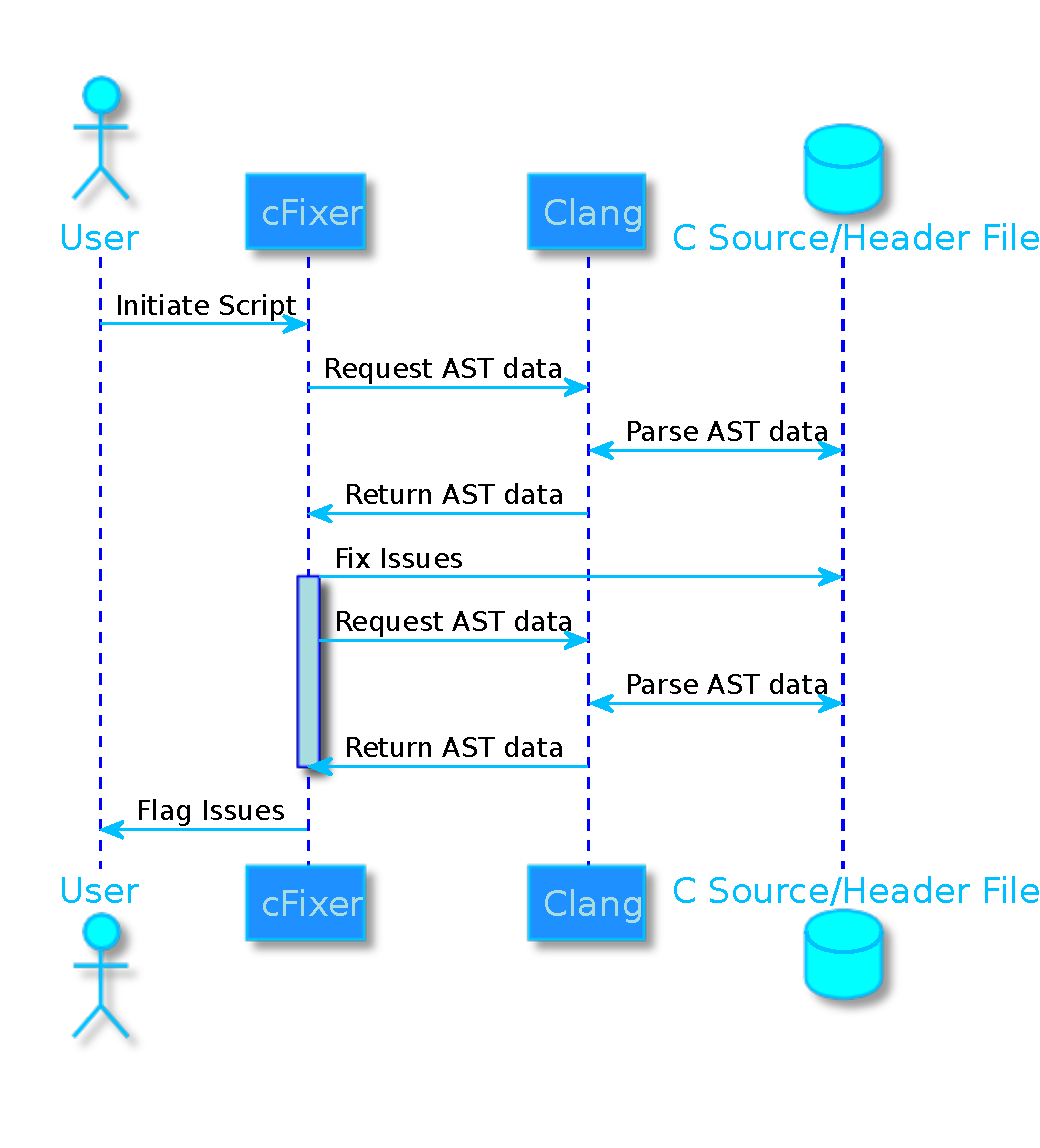
\includegraphics[width=1.2\textwidth]{dataflow}}%
  \label{fig:dataflow}
\end{figure}

\section{User Interface Requirements}

For this product, the user interface will work entirely through the command line, as this is a tool which will be integrated into the compilation and code check-in processes. The tool will take source and configuration files as input and output to either another file or the standard output. Text output should be formatted in a way that is human-readable and relatively easy to parse.

\section{Issues} \label{issues}

Well Defined Issues:
\begin{enumerate}
	\setcounter{enumi}{100}
	\item Inline Comments
	\item In-function Comments
	\item Title Header Comments
	\item Public / Private Trimming
	\item Hard Tabs
	\item Function Headers
	\item File Header Comment Block Indentation
	\item Slash Slash Comments
	\item File Header Comment Block Description Trim
	\item \texttt{NoKeywords} in the File Header Comment Block
	\item File Header Comment Block Copyright Year
	\item Stack Function Arguments in each Parameter List
	\item Brace Alignment
	\item Fix the Casing on
	\item Place Whitespace Around all Parenthesis
	\item Add a Local Variables Section into each Function
	\item \texttt{\#include} Casing, Spacing, Sorting and Ordering
	\item Prototype the Static Functions at the Top
	\item Fix the File Assertion
	\item Precede Newlines with Carriage Returns
	\item Inline Comment Upgrade
	\item Function Order
\end{enumerate}
Other Issues:
\begin{longtable}{p{.50\textwidth} p{.50\textwidth}}
\tabitem Module name not in module header comment & \tabitem Module name in module header comment doesn\'t match\\
\tabitem No description in Module header comment & \tabitem Section is missing, i.e. General Includes, Types\\
\tabitem Section is out of order & \tabitem Section is not centered\\
\tabitem Section comment block not right length & \tabitem Missing design assurance level\\
\tabitem Empty comment block & \tabitem Comment block that extends to 92, these are considered module section comments\\
\tabitem Comment block extends past column 80 & \tabitem Comment blocks top line doesn't match the bottom line\\
\tabitem Local function prototype without the static qualifier & \tabitem Function prototypes out of alphabetical order\\
\tabitem Parameters are not formatted correctly in function prototype & \tabitem Not using void in functions prototypes with no arguments\\
\tabitem Parameter without comment in function prototype & \tabitem Unnecessary comment for function prototype\\
\tabitem Missing function comment header & \tabitem Missing function name in function comment header\\
\tabitem Missing description in function comment header & \tabitem Function comment header extends past column 92\\
\tabitem Missing end of function comment & \tabitem Function name, comment name, and end of comment not all the same\\
\tabitem Unnecessary comment for function itself, the inline one after "void foo(" & \tabitem Parameters not written correctly in function\\
\tabitem No void parameter in empty function & \tabitem Missing comment on function parameter\\
\tabitem Public function out of alphabetical order in module header & \tabitem Non public function in public function section\\
\tabitem Privileged procedures out of alphabetical order in module header & \tabitem Non privileged procedure in privileged section\\
\tabitem Private function out of alphabetical order in module header & \tabitem Non private function in private function section\\
\tabitem Local function in module header out of alphabetical order & \tabitem Non local function in local function section.\\
\tabitem Public function in header that's not in the file. & \tabitem Privileged function in header that's not in the file\\
\tabitem Private function in header that's not in the file & \tabitem Local function in header that's not in the file.\\
\tabitem Public functions not in alphabetical order & \tabitem Function in file that's not in the header.\\
\tabitem Public function not in the public function section of file & \tabitem Privileged function out of alphabetical order\\
\tabitem Privileged function not in the privileged function section & \tabitem Private function out of alphabetical order in file\\
\tabitem Private function not in the private section of the file & \tabitem Local function out of alphabetical order.\\
\tabitem Local variables out of alphabetical order & \tabitem Local variable has no comment\\
\tabitem Standard library includes out of alphabetical order & \tabitem Standard library includes not prior to public private Garmin includes\\
\tabitem Public includes out of alphabetical order & \tabitem Public include not prior to private includes\\
\tabitem Private includes out of alphabetical order & \tabitem Private include not after public includes\\
\tabitem Invalid private includes for component & \tabitem Deprecated "grm\_pub.h" or "grm\_pub\_lib.h"\\
\tabitem Header file not defining multiple include protection & \tabitem Header not looking for multiple include protection\\
\tabitem Headers multiple include protection doesn't match the file name & \tabitem Header missing comment for end of multiple include protection\\
\tabitem Comment at end of file for multiple include doesn't match the defin. & \tabitem Enum has no comment\\
\tabitem Typedef has no comment & \tabitem Typedef members written incorrectly\\
\tabitem Typdef member has no comment & \tabitem compiler\_assert() doesn't match the header file it's used in.\\
\tabitem Function not associated with a c file & \tabitem Function not actually defined in the specified c file\\
\end{longtable}

\bibliography{references.bib}{} \label{bib}
\bibliographystyle{plain}

\section{Glossary}
The following terms are defined in order to provide clarity to the rest of this document:\\

\noindent\begin{tabular}{l p{8cm}}
AST & See \textit{Abstract Syntax Tree}\\
\hline
Abstract Syntax Tree & A tree representation of the abstract syntactic structure of source code in a programming language.\\
\hline
Issue & The problem statement for a syntactic requirement on the C source code structure.\\
\hline
Rule & The code that analyzes, flags, and potentially fixes a specific issue (or a set of related issues).\\
\end{tabular}

\pagebreak
\section{Signatures}
The undersigned parties hereto mutually agree to the validity of statements made within this document. Any modifications to statements within this document must be agreed upon in writing by all signatories and with the consent of the current Senior Software Engineering Project course instructor.
\vspace{.2in}
\SignAndDate{Andrew Stucky (Mentor)}
\vspace{.2in}
\SignAndDate{Nicholas Nelson}
\vspace{.2in}
\SignAndDate{Mark Mills}
\vspace{.2in}
\SignAndDate{Charles Santos}

\chapter{Project Evolution}

\section{Requirements Updates}

Throughout this project, requirements have been revisited and revised as necessary to meet the overarching objectives. The following additions, modifications, and removal of requirements were necessary to successfully complete the project:

\begin{longtable}{| p{.03\textwidth} | p{.32\textwidth} | p{.10\textwidth} | p{.43\textwidth} |}
\hline
1 & cfixer.py unable to run on POSIX-compliant systems (Linux, BSD, OSX, etc.) & Added & Fix merged into \textit{master} branch on Jan 20.\\
\hline
2 & Issue \#110: \texttt{NoKeywords} in the File Header Comment Block & Modified & Client added requirements to remove \$NoKeywords\$, \$Log.\$, \$Id.\$ patterns.\\
\hline
3 & Compatability issue on Cygwin environment & Added & Fix merged into \textit{master} branch on Jan 28.\\
\hline
4 & Issue \#103: Title Header Comments & Modified & Client added requirements to remove deprecated section headers, rename "FILE DO-178B LEVEL" to "DESIGN ASSURANCE LEVEL", added sections headers if they do not exist, and order current and newly inserted section headers in order.\\
\hline
5 & Issue \#108: Slash Slash Comments & Modified & Client removed requirement that slash slash comments be removed when a removal flag is enabled; removal flag option is also removed.\\
\hline
6 & Issue \#116: Local Variables Section & Modified & Client added requirements this solution also handle \texttt{typedefs}, \texttt{const}, and macros.\\
\hline
7 & Issue \#117: \texttt{\#include} Casing, Spacing, Sorting and Ordering & Modified & Client added ANSI standards requirements and dropped Garmin specific standards that contradicted the ANSI standards.\\
\hline
8 & Add issue ordering support & Added & Client added requirement that the production engine allow custom ordering of issue execution.\\
\hline
9 & Updated command-line options & Added & Client added requirement that command-line options support \texttt{+/-c} instead of \texttt{+/-e}.\\
\hline
10 & Remove absolute path dependencies from issue scripts & Added & Client added this requirement to all issues.\\
\hline
11 & Issue \#113: Brace Alignment & Modified & Client added requirement that this issue also handle split statement alignment.\\
\hline
12 & Issue \#123: Empty Comment Block & Added & Client added new issue for removing empty comment blocks, in-line comments, and slash-slash comments.\\
\hline
13 & Issue \#124: Check/Fix Function Footer In-line Comments & Added & Client added new issue for fixing format of in-line comments.\\
\hline
14 & Issue \#125: Check/Fix Header Guard on Header Files & Added & Client added new issue for header guards to conform to \texttt{\_<all caps filename>\_H} format.\\
\hline
15 & Issue \#126: Privileged Function Validation & Added & Client added new issue for detecting public functions and privileged functions existing in the same file; flagging if this is violated.\\
\hline
\end{longtable}

\section{Gantt Chart \& Timeline Updates}

The additions, modifications, and removals to our overall requirements did not force major alterations to our Gantt Chart, but the reduction of our team size from 3 to 2 students prior to the midterm evaluation in Winter 2015 required modifying the timeline for our releases in order to accomodate completing the same requirements with a reduced workforce.

See Figure~\ref{fig:versioning} for the illustration of our release model.
See Table~\ref{original_release_schedule} and Table~\ref{updated_release_schedule} for the updates to our release schedule, and Figure~\ref{fig:timeline} for the timeline from \textit{Microsoft 365} site used to manage the project.
The Gantt Chart for the project is included in Figure~\ref{fig:gantt}.

\begin{longtable}{| p{.20\textwidth} | p{.45\textwidth} |}
\caption[Original Release Schedule]{Original Release Schedule} \label{original_release_schedule} \\
\hline
December 8 & Version 1.0 released\\
\hline
March 13 & Version 2.0 released\\
\hline
May 8 & Version 3.0 released\\
\hline
May 15 & EXPO Event\\
\hline
\end{longtable}

\begin{longtable}{| p{.20\textwidth} | p{.45\textwidth} |}
\caption[Updated Release Schedule]{Updated Release Schedule} \label{updated_release_schedule} \\
\hline
December 19 & Version 1.0 released\\
\hline
March 24 & Version 2.0 released\\
\hline
May 12 & Version 3.0 released\\
\hline
May 15 & EXPO Event\\
\hline
\end{longtable}

\begin{figure}[ht]
  \caption{Project Timeline}
  \makebox[\textwidth][c]{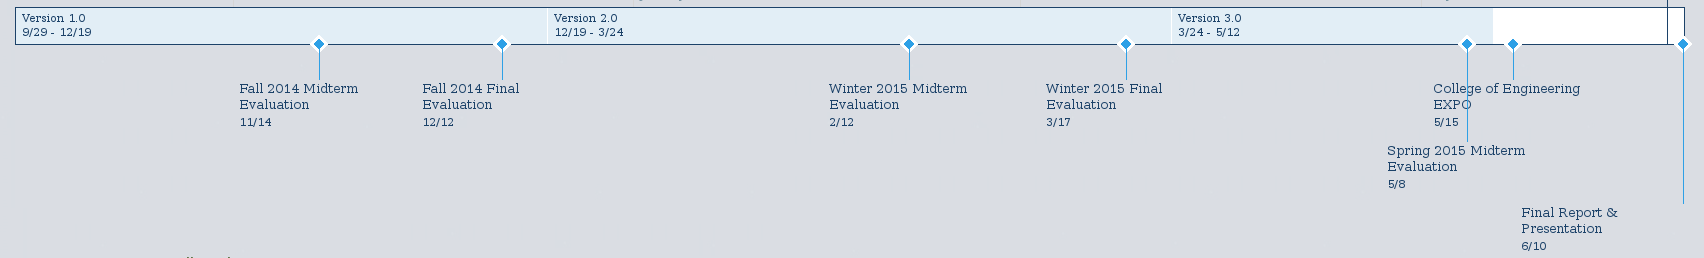
\includegraphics[width=1.1\textwidth]{timeline}}%
  \label{fig:timeline}
\end{figure}

\begin{figure}[ht]
  \caption{Gantt Chart}
  \makebox[\textwidth][c]{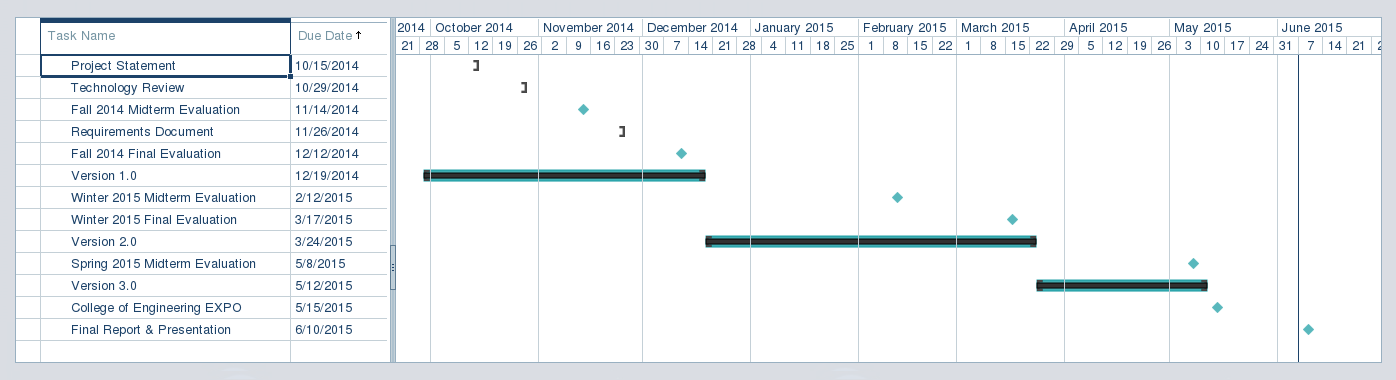
\includegraphics[width=1.1\textwidth]{gantt}}%
  \label{fig:gantt}
\end{figure}

\chapter{Weekly Blog Posts}

\section{Analyzing the Problem}
\textit{Friday, November 7, 2014 by Nicholas Nelson}
\newline

All other classwork aside, we have begun to get into the specifics of our project and where appropriate goals and boundaries should be set. I have previous experience using Abstract Syntax Trees (AST) in Java during a summer research assistantship with a team of graduate student researchers at OSU. Capitalizing on that experience, we have begun to explore the capabilities and limitations of AST constructs in the C language. As a team, we have agreed to watch the 45 minute video that introduces the LLVM project's Clang infrastructre, including the Clang AST parser, on their website: \textit{http://clang.llvm.org/docs/IntroductionToTheClangAST.html}.

\section{Requirements Pinned Down}
\textit{Friday, November 21, 2014 by Charles Santos}
\newline

This week, we finalized our requirements document. It is likely the largest assignment and compilation of information about our project so far (and probably going forward for a while) because it describes absolutely everything about the project.
The detail is necessary because, firstly, this is the explicit definition of what our customer will be receiving and, secondly, it defines what we will be delivering at each release.
If nothing else, I think that getting all of this information together, while involved and a bit tiring, is very exciting because it is the first glimpse at what our finish product will look like.

\section{Holiday}
\textit{Friday, November 28, 2014 by Charles Santos}
\newline

With Thanksgiving this week, all we had to do was get the requirements document absolutely finished, signed, and handed in. In the end, it was a respectable stack of paper and, I think, turned out well.
I don't konw about the other members of the group, but my family was very interested in my capstone project and while it will be a lot of work, I am glad that I can be involved in such a large and \"real-worldly\" project.

\section{Winter Term has begun!}
\textit{Saturday, January 10, 2015 by Nicholas Nelson}
\newline

As a team, we attempted to mix code development with our holiday break in order to get a jump on our upcoming milestones. We had only mild success with that though. Mainly due to travels and other time commitments. We did get started on two issues from the list of coding standards issues that were identified in our Requirements Document.

We had our biweekly teleconference meeting with Andrew and determined that completely 6-8 issues this week was not feasible or likely, so we pushed version 1.0 back to Friday, January 23 release date. We should have a code freeze on Wednesday, January 21 in order to allow time for Andrew to conduct a code review.

\section{Week 2 of Winter Term}
\textit{Thursday, January 15, 2015 by Nicholas Nelson}
\newline

After getting settled into classes, we have begun to outline which issues we will be focusing on throughout the rest of the term. We have mainly focused on the top 20-30 issues identified in our list that was provided by our sponsor, since those have a higher priority.

\section{Week 3 and Release 1.0}
\textit{Friday, January 23, 2015 by Nicholas Nelson}
\newline

We had originally planned to release 1.0 on Friday, but since only 2 issues have been implemented and reviewed we decided to postpone version 1.0 until an additional 4-6 issues can be checked into github. Andrew indicated that we need to begin developing implementation code at a faster pace in order to meet our intended requirements.

\section{Week 4}
\textit{Wednesday, January 28, 2015 by Nicholas Nelson}
\newline

This week has mostly been comprised of iterative development cycles on 4-5 issues that we have been working on individually. We have had to clarify some of the scope of individual issue requirements, and fix bugs in the testing framework in order to proceed.

\section{Week 5}
\textit{Sunday, February 8, 2015 by Nicholas Nelson}
\newline

Further development work has seen 4 out of 5 in-progress issues fully completed and merged into the master branch of the git repository. With the completion of the remaining open issue, we should have enough for releasing Version 1.0.

Some of the stumbling blocks have been specific details of the requirements of specific issues. For example, an issue that originally required locating all instances of a keyword within the input C file and either removing or adding it to the appropriate location within the file. After further discussion, the requirements were changed to only require locating and removing the keywords. Additional development time was spent developing a dynamic adding function that was not required in the end.

\section{Week 6 and Version 1.0}
\textit{Wednesday, February 11, 2015 by Nicholas Nelson}
\newline

Resolving the final outstanding issue has allowed us to provide the customer with a complete set of issue solutions for validation and integration into the master branch. Andrew (our customer) merged and released Version 1.0 on Wednesday, February 11, 2015.

We are now beginning work on solutions to 8-10 issues for inclusion in Version 2.0. Further discussion and development will occur during our biweekly teleconference meeting with Andrew on Friday.

\section{Week 7}
\textit{Wednesday, February 19, 2015 by Nicholas Nelson}
\newline

Only 3 issues have been resolved to the point of submitting pull requests for Andrew to review and merge. Upon examining the issues we currently have assigned to version 2.0, it is clear to us that these issues will require more extensive development in order to meet the requirements. Several issues require heavy use of the full API for Clang AST or in-depth Python and regular expression evaluations in order to locate affected areas in the target files and test files.

In some issues we have hit a snag based on the capabilities of our current APIs and libraries, and we are having to develop shared code for determining things like function signatures, types of comment blocks, sections within comment blocks (which Clang AST considers to be a singular \textit{comment block} node), etc.

\section{Week 8}
\textit{Wednesday, February 25, 2015 by Nicholas Nelson}
\newline

Several complex code blocks for issues that are outstanding for version 2.0 have seen major progress this week. We spent our biweekly phone meeting with Andrew discussing details to some of these issues and clarifying the expected results that Garmin expects from each. There was only 1 pull request for a finalized issue this week, but that was not indicative of the progress that was made. Now that midterms are over we can hopefully get the rest of version 2.0 up and running.

\section{Week 9}
\textit{Friday, March 6, 2015 by Nicholas Nelson}
\newline

Because coursework for our other classes has been demanding in light of the upcoming end to the term, our development pace has slowed a bit. We had 2 pull requests, but one was immediately rejected because it breaks on Andrew's test runs. We are also working on the status report for the Winter 2015 term in order to have it ready for final evaluation.

Some re-engineering in order to maintain cross-platform support was required and held up further work on the issue solutions until Andrew Stucky and Nick Santana could weigh in and provide the necessary file inclusions. They were very quick with the updates, but it did hold up some development.

\section{Finals Week}
\textit{Monday, March 16, 2015 by Nicholas Nelson}
\newline

Unfortunately we did not have a chance to meet and discuss any of our current work on version 2.0 issues during Week 10. With the demands of all of our other classes, we have slipped on our schedule and asked Andrew for permission to update the version 2.0 release date to Friday, March 20, 2015. We are hoping to finish the rest of the 6 open issues between now and then so that we can proceed with version 3.0 issues.

\section{Spring Break \& Spring 2015 Term}
\textit{Wednesday, March 25, 2015 by Nicholas Nelson}
\newline

Charles was able to complete all of his version 2.0 issues prior to our previously set March 20 release date. But I unfortunately got bogged down with issue 112 and after 60+ hours of development time it was decided to shift this issue to version 3.0 and move onto the other two outstanding issues (102 and 103). We also agreed to move forward with version 2.0 being released on Tuesday, March 24, 2015.

Both Charles and I used our Spring Break vacations to work on this project when we could, but travel and vacations meant that we were only able to work in stop and start sessions. We had 7 pull requests within the last 2 weeks, so we are continuing to move forward.

\section{Week 1}
\textit{Sunday, April 5, 2015 by Nicholas Nelson}
\newline

After reviewing our version 2.0 release and the open issues that have not yet been resolved, we determined that some additional issues could be added to fix some of the infrastructure issues that have cropped up; specifically around locating comment blocks and replacing text when located using regular expressions. With new classes starting we have only had 1 pull request submitted so far.

\section{Week 2 \& 3}
\textit{Tuesday, April 14, 2015 by Nicholas Nelson}
\newline

With the midterm evaluations coming up soon, we have spent this week developing code for our individual issues that will be used for the requirements evaluations. We did not submit any pull requests, but lots of code commits can be found in our \textit{git} repositories.

\section{Week 4}
\textit{Friday, April 24, 2015 by Nicholas Nelson}
\newline

Several graduation oriented events have occurred in the last week or two, and this has taken some of our attention away from the project. We regrouped for a brief team meeting after our check-in with Nels Oscar (TA), and were able to make sure that we are prepared for releasing version 3.0 in two weeks. We still have 10 issues that need to be finished prior to that release.

\section{Week 5 \& Midterm Requirements Evaluation}
\textit{Tuesday, April 28, 2015 by Nicholas Nelson}
\newline

Charles was able to have Nels evaluate his completed requirements for the midterm point of the Spring 2015 term, but I have had to postpone my evaluation until Friday because of issue 112. This issue continues to become more complicated and troublesome, but I believe a complete refactoring over the weekend means that I will be able to finish it soon.

We submitted 4 pull requests either over the weekend or yesterday, so we are still making progress.

\section{Week 6}
\textit{Thursday, May 7, 2015 by Nicholas Nelson}
\newline

Some midterms in other classes were cause for development to be slow this week. We only did 2 pull requests, but now that issue 112 is done I am able to move forward with my remaining issues. Version 3.0 might have to be pushed back since we still have 4 issues outstanding and we were suppose to have the release tomorrow. We will be discussing this issue with Andrew during our biweekly conference call tomorrow. Obviously it can't be pushed back too far since EXPO is next Friday.

\section{EXPO!!!}
\textit{Thursday, May 14, 2015 by Nicholas Nelson}
\newline

Our poster is printed and ready, all issues for version 3.0 have been pulled into the \texttt{master} branch, and we have dress shirts and ties on standby. Our booth is located on the 4th floor near the stairwell on the eastern end of Kelley Engineering Center. Tomorrow is the College of Engineering EXPO!

\section{Project Conclusion}
\textit{Friday, June 5, 2015 by Nicholas Nelson}
\newline

We had a successful presentation at EXPO, but did not receive much traffic due to our location. We met with Nels Oscar for the last time a few weeks ago and according to him we have met all expectations and requirements other than the final report and video presentation. We also had a brief meeting with Andrew Stucky, our mentor/sponsor from Garmin AT, during the EXPO and he expressed that we had done a good job and that the final product was beginning to be adopted by several development teams within Garmin. The response from those teams has been positive.

We would like to thank Andrew for his support and time on this project, Nick Santana for his technical expertise, Nels Oscar for his assistance and timely input, and Kevin McGrath for leading a productive and encouraging senior software engineering course.

\chapter{EXPO Poster}

\chapter{Project Documentation}

Since our project involves modifying source code files for developers, the cfixer application provides a command-line interface (CLI) for ease-of-use, portability, maintenance, and scripting extensibility.
The technical skillset of intended userbase allowed us to forgo development of a graphical user interface (GUI) and focus primarily on providing bullet-proof executions that can be scripted using user-defined config files.

The \texttt{cfixer} application is composed entirely in Python, specifically compatible with Python 2.7.10 (but capable of running with Python 2.7.x or 3.4.x versions), and encapsulating the LLVM project's Clang AST libraries\footnote{http://clang.llvm.org/}, specifically Clang 3.7 (written in C++ and compatible with C, C++, Objective-C and Objective-C++ programming languages).
Because it utilize lambda functions, anonymous functions, and newer regular expression libraries (\texttt{regex}) in Python, \texttt{cfixer} is not compatible with Python 2.2 or older version\footnote{https://docs.python.org/2/whatsnew/2.2.html}.

The \texttt{cfixer} 1.0 application introduced cross-compatible infrastructure, which was further updated in version 2.0, so that it can be run on Microsoft Windows, Apple OSX, Cygwin, and Linux/Unix-like systems (Ubuntu, Debian, GNU, BSD, etc.).
Additional systems that support and are capable of running Python 2.7+ code could be compatible with \texttt{cfixer}, but they have not been tested at this time.

\section{Installation}

\textbf{Prerequisites}
\begin{itemize}
	\item Python 2.7.x or 3.4.x
	\item Terminal access (\texttt{Cygwin} for Windows is recommended)
	\item Local clone of \texttt{GarminAT/osu-code-check-2014} repository
\end{itemize}

As a proprietary product of Garmin AT Inc., the \texttt{cfixer} application is not publicly available.
The source code is maintained in a private \texttt{git} repository that must be cloned and run locally.
For development purposes during this project, code has also been maintained on GitHub\footnote{https://github.com/} in a private repository accessible to the project team.

Python 2.7+ must be installed prior to running the \texttt{cfixer} application, and the installation process for that environment is highly-specific to the operating system. Consulting the Python download pages\footnote{https://www.python.org/downloads/}, including installation instructions, for your specific system is the preferred method.

Since all interaction with the \texttt{cfixer} application occurs in the terminal, no installation process is required directly for \texttt{cfixer}.

\section{Usage}

\texttt{cfixer} can be executed in two ways; through direct command-line execution, or scripted in config files that contain the same CLI commands.
Since both methods invoke the \texttt{cfixer} application through command-line execution, this guide will focus on individual commands.
Any commands highlighted can also be included in a config script for chaining commands.

The first thing to consider when running \texttt{cfixer} is “Which issues do I want to run?”.
Issues are the modular scripts which encapsulate the checking and fixing functionality related to a single rule.
A simple example of an issue is the one which converts tabs to four spaces.
This issue can accept an argument for the number of spaces used in the conversion, but this defaults to four.
A more complex issue is one which aligns and organizes the contents of the parameter list in a function signature.
This list can include the parameter names, their types, qualifiers and comments in a number of places.
Each issue is referred to by its number, so for example, the tab conversion issue is 105 and the parameter alignment one is 112.

After deciding which issues to run, it is really quite easy to run \texttt{cfixer}. With the source installed correctly, it is just a matter of invoking Python with \texttt{cfixer} as the first argument, followed by any number of issue commands and their appropriate number of arguments. 
A typical invocation of \texttt{cfixer} will appear similar to the following:\\
\lstset{language=Python}
\begin{minipage}{\linewidth}
\begin{lstlisting}[frame=single,basicstyle=\small]
python cfixer.py stdout \path\file.c +c112 +f105 5	(Windows)
or
./cfixer.py stdout /path/file.c +c112 +f105 5		(Linux)
\end{lstlisting}
\end{minipage}

The \texttt{stdout} parameter tells \texttt{cfixer} to use the standard output (output to the screen).
This is another modular aspect of the product which allows \texttt{cfixer} to be integrated into the build pipeline of IDEs.
Other output modules exist that interact with Eclipse and Visual Studio’s outputs, though we did not work on this aspect of the product.
\texttt{file.c} is simply the input file which we will be checking against and fixing (only where the \texttt{+<issue>} option is used). 
Finally, the rest of the command is the arguments to \texttt{cfixer}.
\texttt{+c112} indicates that we want to run issue 112 in check mode, meaning it will look for errors but not correct them.
\texttt{+f105 5} indicates that we want to run issue 105 in fix mode, meaning errors will be found and fixed in the file, and the 5 is an argument to the issue coming before it, in this case specifying that we want to replace any tabs with 5 spaces.
In addition to the above usage, one can invoke \texttt{cfixer} using a config file similar to the following:\\
\lstset{language=Python}
\begin{minipage}{\linewidth}
\begin{lstlisting}[frame=single,basicstyle=\small]
python cfixer.py \path\file.c @config.cfg		(Windows)
or
./cfixer.py stdout /path/file.c @config.cfg		(Linux)
\end{lstlisting}
\end{minipage}

This invocation is nearly exactly the same as above, except the issue list and arguments are in a config file, \texttt{config.cfg}, allowing for projects to save and commit their test configurations.

\section{Structure \& Design}

Under the surface, the operation of \texttt{cfixer} is also quite straightforward.

Upon invoking \texttt{cfixer}, the first thing that happens is the list of issues are compiled together, reordered such that they will not interfere with each other, and the issue objects are instantiated with their specific parameters.
At this point, the issue objects accept the target file(s), one at a time, in the order specified above.
Before the issue examines the target file, the Clang interpreter is invoked to build the abstract syntax tree (AST) representation of the file.
Depending on the specific issue invoked, the Clang interpreter might also be tasked with tokenizing and serializing the file for more detailed evaluations.
At this point, the issue is handed the execution thread and can begin examining the file for specific violations that should be flagged or fixed (as indicated).

The implementation of each issue is unique, but at a high level, the issue first identifies problematic tokens and/or blocks of code that do not meet the specific requirements for that issue and are then reported to standard output (\texttt{stdout}) or any other \textit{Reporter} indicated, and/or fixed through specific resolution steps indicated in the issue code.
Upon sucessful completion of an issue, it hands execution thread control back to the \texttt{cfixer} application and the next issue (if any) is executed.
Because the state of the target file is not fixed, and highly volatile when fixes are applied, each issue that executes must regenerate the AST representations prior to executing it's own check and/or fix code.

\section{Theory of Operation}

The \texttt{cfixer} application utilizes a modular infrastructure of isolated solutions that accept AST representations (typically in the form of serialized token mappings) and string representations (through reader/writer APIs) of the target file.

This design allows for a plug-and-play system that can easily be maintained by removing unnecessary, redundant, or depreciated issues and adding new issues as needed.
To further the portability of \texttt{cfixer}, the reporting processes of the system are encapsulated in \texttt{Reporter} class files that can also be added to and removed as needed.
Although not highlighted in this project, the intent of this project is to eventually pipeline the process of reviewing and fixing code formatting issues as part of the typical product build process.
Capturing error messages and status outputs are thus highly desirable, and future work will focus on developing the necessary \texttt{Reporter} classes to enable this type of execution.

\section{API Documentation}
Since \texttt{cfixer} will continued to be developed by Andrew Stucky and his team, the current state of the \texttt{cfixer} API is not permanent and most likely guaranteed to change as furthe development code is added to the project.
Although some functions and classes have been properly documented through \texttt{pydoc} documentation comments within the Python code, not all issues contain complete and accurate comments, and should thus be read with a grain of salt.

A partial documentation of the \texttt{cfixer\_util} infrastructure file can be found by generating and reviewing the \texttt{pydoc} from the \texttt{doc/source/index.rst} or directly reviewing the code (which includes several in-line comments).
Also, some of the infrastructure central to the \texttt{cfixer} application is taken from the \textit{Clang AST} libraries and can be consulted by visiting:
\url{http://clang.llvm.org/doxygen/}.

\chapter{New Technologies \& Reference Materials}

\section{Web Resources}
The majority of our design work occurred during the Fall 2014 term and was documented in the Original Client Requirements Document that is outlined in Chapter~\ref{orig_req_doc}.

Since our project was developed in Python, and highly dependent on the structure and standards of C, we obviously spent a significant amount of time referencing the Python and C language documentation available online.

\begin{itemize}
	\item Python 2.x documentation: \url{https://docs.python.org/2/}
	\item C documentation: \url{http://en.cppreference.com/w/}
\end{itemize}

\section{Reference Books}

All of the books, research papers, and references that were used during the design and development of this project can be found in the bibliography contained in Section~\ref{bib}.

\chapter{Learning Outcomes}

\section{Outcomes for Charles Santos}

\subsection{What technical information did you learn?}

The technical skills that I learned from this project were mostly having to do with Python itself and Clang.
Before this, my experience with Python was rather limited, having only used it in one previous course.
Now, I feel like I have a much stronger intuitive idea of how to do things in Python and how to leverage some of its more complex and unique capabilities.

In contrast, I am still quite hazy when it comes to Clang.
Since we were limited to Python bindings on a C library, we could not access all of the information and functionality Clang had to offer and even then, a great deal of the capabilities of the library were shrouded by the bindings.
For a few issues, I tried to work with Clang directly through the bindings and referred to the library's documentation, but the capabilities available in C were just not similar enough to what I was seeing in Python to make any sense.
To overcome this, I used the premade functionality that leveraged the AST, specifically some helper functions that just pulled out specific areas of the file like function definitions and went from there.

\subsection{What non-technical information did you learn?}

The first non-technical aspect of this project that I can think of was working working as a member of a real team.
This was not my first time working in a more professional, ``real world'' environment, but it had been a little while since the last time I had been in one.
Communication between the various people involved in the project was very common and I had to get back into the mindset of ``business communication'', focusing on succinctness and clarity in my messages.

\subsection{What have you learned about project work?}

Like I mentioned above, this was not my first time working in a more serious manager-developer sort of team project, so the whole situation was familiar to me.
In this case, however, there were definitely a few times the client asked for some tasks to be implemented in specific ways that I did not agree with and whereas before I could say ``as the technical decision maker here, I am vetoing your decision'', but with this client I could not.

\subsection{What have you learned about project management?}

Again, the above two sections cover this fairly well.
I will say that having a project manager who is familiar with software development is infinitely more valuable and, in my opinion, capable than one who just has a creative idea and no sense of how to implement it.
In this case, our client was very knowledgeable and helpful and made the project much more doable.

\subsection{What have you learned about working in teams?}

Working in a small team like this with a project that was easily divided up between the two of us, I think we had a pretty easy time.
Compared to some of the other projects, I think that the scope of our tasks made for easy planning and flexible schedules.
Similarly, I am very grateful that my teammate was as knowledgeable, useful, and friendly as he was.
In the past, I have been in the opposite situation, so I have learned how much of a difference that can make.

\subsection{If you could do it all over, what would you do differently?}

I think that my experience overall was really very near to optimal.
The only thing I could complain about is how mundane formatting C code is, but that does not even come near spoiling the experience.


\section{Outcomes for Nicholas Nelson}

\subsection{What technical information did you learn?}

Having previously developed industrial process automation software during a summer internship at Hewlett-Packard in the summer of my sophomore year, I already had experience in Python development and Python-style scripting. During the summer of my junior year, I also had a undergraduate research assistant position that involved software engineering with abstract syntax tree (AST) libraries in Ruby and Java. But since neither of those technologies were combined, and I didn't have an opportunity to work with the Clang AST libraries until now.
The biggest new technologies were related to the problems of syntax evaluation and processing using ASTs and regular expressions.

The most difficult technical subject matter that I learned during this project had to do with functional programming elements within Python; namely, lambda expressions, anonymous functions, and recursive iteration functions. Some of the underlying conceptual understanding came from also taking the CS444 Operating Systems II, CS480 Translators, and CS381 Programming Languages courses during this project.

\subsection{What non-technical information did you learn?}

Having been in many projects within the Information Technology (IT) sphere during the 5 years that I worked at Samaritan Health Services within their IT department, my understanding of technical projects was already present. But having the opportunity to work on a complete end-to-end software engineering and development project was a new experience for me. Managing coding deadlines that were not directly tied to course assignments was enlightening and single biggest lesson that I learned was that it is best to "under promise, over deliver" within the software development world. Managing time constraints becomes critical when the mysteries of software solutions are not self-evident when planning.

\subsection{What have you learned about project work?}

Project work is always a mystery when going into it, typically becoming even murkier once you're embroiled in it, but once the end is near and there is time to reflect I see that learning to over-design at the onset and keep your head down and working once it's time to put that plan into action is essential to keeping the momentum of a project moving forward.
The only caveat that I have to that rule though, is that at regular intervals during the timeline of a project, the overall health and direction of the project should be assessed with all stakeholders involved. Nothing is more troubling than finding out that the clients have switched gears and would like to pivot the potential uses for a project into something bigger and more complex.

\subsection{What have you learned about project management?}

Although I have a lot of experience both in corporate projects, IT projects, and school projects, I continue to receive reinforcement that I would rather not become a project manager. I enjoy organizing people and projects at the team level, but multi-departmental multiple stakeholder projects seem to become myried in the differences between technically adept and non-technically aware members of these types of teams.

\subsection{What have you learned about working in teams?}

The loss of one of our teammates at the midpoint of the project actually enabled us to more swiftly complete the tasks that needed to be completed.
But reflecting on this change, I am reminded that every member of a team has their own motivations and goals for participating in the team.
They may appear to be focused on the project, but other forces outside of my control can also be at play, and understanding these elements (or at least being prepared for them) is the best way to maintain an even keel within a team.

\subsection{If you could do it all over, what would you do differently?}

I would insist to the client that building a shared infrastructure of functions and code that can be reused by every member of the team is a highly desirable trait within a modular project such as this one. Other than that, I would generally stick to the same game plan.

\chapter{Appendices}

\section{Essential Code}

\subsection{cfixer.py}
\lstset{language=Python,breaklines=true}
\begin{lstlisting}[frame=single,basicstyle=\small]
#!/usr/bin/env python
#-*- encoding: utf-8 -*-
""
:mod:`cfixer` --- Autofixer for code files
===========================================
Auto-fixes conventional errors within the file this file is called upon.
There are options to check or fix all errors and formatting.
""

import sys
import string
import os
import pprint
import argparse
import logging
import copy
from pprint import pprint
from sys import platform as _platform

current_dir = os.path.dirname(os.path.abspath(__file__))
parent_dir = os.path.dirname(current_dir)

#--------------------------------------------
#Owing to the fact that this isn't a package, this
#block makes it possible for us to relatively import
#other units of code.
if __name__ == "__main__" or __package__ is None:
    mod_name = os.path.basename(current_dir)
    sys.path.insert(1, parent_dir)
    mod = __import__(mod_name)
    sys.modules[mod_name] = mod
    __package__ = mod_name
#---------------------------------------------
#Must be below the above section of code.
import walker
from .clang import cindex
from .clang.cindex import Config
from .clang.cindex import Index
from .clang.rewriter import Config as rewriter_config
from .clang import rewriter
from .issue_checkers import *
from .reporters import *
from cfixer_base import *
from cfixer_util import *

ISSUE_CLASS_PREFIX = "Issue"
REPORTER_MODULE_SUFFIX = "_reporter"
ISSUE_MODULE_PREFIX = __package__ + ".issue_checkers.issue"
REPORTER_MODULE_PREFIX = __package__ + ".reporters."

class CommentArgParser(argparse.ArgumentParser):
    ""
    Basic argparser in addition to giving the ability to skip over comments with
    a custom denotation in the config file/arg list.
    ""
    def __init__(self, *args, **kwargs):
        super(CommentArgParser, self).__init__(*args, **kwargs)

    def convert_arg_line_to_args(self, line):
        for arg in line.split():
            if not arg.strip():
                continue
            if arg[0] == "#":
                break
            yield arg


class IssueAction(argparse.Action):
    ""
    This handles processing of the issue flags as provided by the argparser.
    This will verify the arguments passed with the issue type flag, and if successful will
    append the issue checker/fixer to the list.
    In order to extend the list this needs to do a deep copy of the list and then add the
    new item to the deep copy, and finally set the stored list to the new copy.
    This assumes the default is set to [], probably need to make a copy of argparse.py
    _ensure_value()
    ""
    def __call__(self, parser, namespace, values, option_string=None):
        if option_string.startswith("+f"):
            fix_item = True
        elif option_string.startswith("+c"):
            fix_item = False
        #---------------------------------------------
        #This block adds functionality for subtracting out fixers/checkers from
        #the command line.
        elif option_string.startswith("-f") or option_string.startswith("-c"):
            all = string.maketrans('', '')
            nodigs = all.translate(all, string.digits)
            cline_issue_str = option_string
            cline_issue_str = cline_issue_str.translate(all, nodigs)
            for each_instantiated_issue in getattr(namespace, self.dest):
                class_type = type(each_instantiated_issue).__name__
                ref_prefix = str(class_type).translate(all, nodigs)
                if ref_prefix == cline_issue_str:
                    getattr(namespace, self.dest).pop(getattr(namespace, self.dest).index(each_instantiated_issue))
            return
        #---------------------------------------------

        #Parse the reporting arg from the command line, instantiate it, and prepare
        #to pass it into the newly instantiated issue object.
        reporter_label = getattr(namespace, "reporter") + REPORTER_MODULE_SUFFIX
        reporter_class = getattr(sys.modules[REPORTER_MODULE_PREFIX + reporter_label], reporter_label) #Issue is in second argument
        reporter_instance = reporter_class()

        #Instantiates the issue object with prepared arguments.
        issue_num = option_string[2:]
        issue_cls = getattr(sys.modules[ISSUE_MODULE_PREFIX + issue_num], ISSUE_CLASS_PREFIX + issue_num)
        new_issue = issue_cls(fix_item, issue_num, values, getattr(namespace, "source_file"), reporter_instance)

        issues = copy.copy(getattr(namespace, self.dest))
        issues.append(new_issue)
        setattr(namespace, self.dest, issues)

class ChunkMaster(object):
    ""
    Dedicated to chunking the file into usable sections with the use
    of the libclang API.
    ""
    def __init__(self, file_name, file_folder_root, clang_options=None):
        args = None
        args = get_sub_directories(get_file_root_dir(os.path.abspath(os.path.dirname(file_name))))
        args.append("-I" + os.path.dirname(os.path.abspath(__file__)) + "/clang/include")
        # dynamic library linking on POSIX-compliant systems (Linux, BSD, OSX) require .so linker files, whereas
        # Windows systems utilize .dll linker files
        clang_lib = None

        if _platform == "win32" or _platform == "cygwin":
            clang_lib = os.path.dirname(os.path.abspath(__file__)) + "/clang/libclang.dll"
        else:
            clang_lib = os.path.dirname(os.path.abspath(__file__)) + "/clang/libclang.so"
        cindex.Config.set_library_file(clang_lib)
        rewriter.Config.set_library_file(clang_lib)
        opts = cindex.TranslationUnit.PARSE_DETAILED_PROCESSING_RECORD | cindex.TranslationUnit.PARSE_PRECOMPILED_PREAMBLE

        # handle both relative and absolute paths
        abs_file_name_path = ''
        if os.path.isabs(file_name):
            abs_file_name_path = file_name
        else:
            abs_file_name_path = os.path.dirname(os.path.dirname(os.path.abspath(__file__))) + '/' + file_name

        with open(abs_file_name_path, "rb") as source:
            source_file = source.read()
        # FIXME: Not sure why clang seems to be holding onto the file on some PCs. So read
        # the file into memory and pass it to clang that way.
        self._tu = cindex.TranslationUnit.from_source(file_name, args, [(file_name, source_file)], opts)
#        cr = self._tu.codeComplete(file_name, 9, 1, include_brief_comments=True)
        self._cursor = self._tu.cursor
        self._file_name = file_name
        self._rewriter = rewriter.Rewriter.from_tu(self._tu)

        # HACK, use this to print out the clang errors
        for diag in self._tu.diagnostics:
            print diag

    def __node_in_main_src_file(self, node):
        ""

        :param node: The node to check for being in a source file.

        :type node: An AST node or even a token, it just needs to have a SourceLocation at its location property.

        This function returns True if the node is one in the main source file.
        ""
        try:
            return node.location.file.name == self._file_name
        except AttributeError:
            return False


    def get_file_location(self, line, column):
        ""

        :param line: the desired line in the file

        :type line: integer

        :param column: the desired column on the line

        :type column: integer

        Get the location for the given line and column

        ""
        return cindex.SourceLocation.from_position(self._tu,
                                                   self._tu.get_file(self._file_name), line,
                                                   column)
    def get_next_func_decl(self):
        ""
        This will iterate through all function declarations, this includes the declaration
        body as part of an actual function definition.
        ""
        for node in self._cursor.get_children():
            if self.__node_in_main_src_file(node) and \
                    node.kind == cindex.CursorKind.FUNCTION_DECL:
                # We have a function declaration, so we need to find where the compound
                # statement starts, if it has one, and end the source range there.
                end = node.extent.end
                for child in node.get_children():
                    if child.kind == cindex.CursorKind.COMPOUND_STMT:
                        end = child.extent.start
                        break

                yield FileChunk(self, node, cindex.SourceRange.from_locations(node.extent.start,
                                                                              end))

    def get_tokens(self, extent=None):
        ""

        :param extent: extent to get tokens for, if extent is none then it will get tokens for the entire file

        :type extent: cindex.SourceRange

        This will return generator for the tokens in the given extent.
        ""
        if not extent:
            extent = self._cursor.extent

        return self._tu.get_tokens(extent=extent)

    def chunkify_statements(self, src_file):
        ""

        :param src_file: File input to be chunked

        :type src_file: string

        Parses the source file, finds the root directory for the project,
        adds in all includes, and divides the file into chunks suitable
        for easy programmer use. Currently divides into
        Fors
        Structs
        Typedefs
        Fucntions
        Preprocessor statements
        Whiles
        Variable declarations
        Returns
        Cases
        Switches
        Enumerations
        Ifs
        Macros
        Parameters
        Dos
        ""
        return_list = []
        def get_children_recursive_helper(self, over_node):
            if len(list(over_node.get_children())) > 0:
                for child in over_node.get_children():
                    return_list.append(over_node)
                    get_children_recursive_helper(self, child)
            else:
                return_list.append(over_node)

        def get_children_recursive(self):
            for node in self._cursor.get_children():
                if self.__node_in_main_src_file(node):
                    get_children_recursive_helper(self, node)

        for_statements = []
        struct_statements = []
        typedef_statements = []
        function_statements = []
        preprocessor_statements = []
        while_statements = []
        var_statements = []
        return_statements = []
        case_statements = []
        switch_statements = []
        enum_statements = []
        if_statements = []
        macro_statements = []
        param_statements = []
        do_statements = []
        compound_statements = []
        #A function or method parameter.
        get_children_recursive(self)
        #There are more attributes to be pulled from here
        #http://www.masella.name/~andre/libgit2/libclang/Clang.CursorKind.html
        #There are many, many more.

        #Yes, this is an ugly way to do this. However, it is the fastest and the use
        #of this class comprises the largest percentage of time used by this
        #program.
        for each in return_list:
            if each.kind == cindex.CursorKind.FOR_STMT:
                for_statements.append(each)
            if each.kind == cindex.CursorKind.STRUCT_DECL:
                struct_statements.append(each)
            if each.kind == cindex.CursorKind.TYPEDEF_DECL:
                typedef_statements.append(each)
            if ((each.kind == cindex.CursorKind.FUNCTION_DECL) and (each.type.kind == cindex.TypeKind.FUNCTIONPROTO)):
                function_statements.append(each)
            if each.kind == cindex.CursorKind.INCLUSION_DIRECTIVE:
                preprocessor_statements.append(each)
            if each.kind == cindex.CursorKind.WHILE_STMT:
                while_statements.append(each)
            if each.kind == cindex.CursorKind.VAR_DECL:
                var_statements.append(each)
            if each.kind == cindex.CursorKind.RETURN_STMT:
                return_statements.append(each)
            if each.kind == cindex.CursorKind.CASE_STMT:
                case_statements.append(each)
            if each.kind == cindex.CursorKind.SWITCH_STMT:
                switch_statements.append(each)
            if each.kind == cindex.CursorKind.ENUM_DECL:
                enum_statements.append(each)
            if each.kind == cindex.CursorKind.IF_STMT:
                if_statements.append(each)
            if each.kind == cindex.CursorKind.MACRO_DEFINITION:
                macro_statements.append(each)
            if each.kind == cindex.CursorKind.PARM_DECL:
                param_statements.append(each)
            if each.kind == cindex.CursorKind.DO_STMT:
                do_statements.append(each)
            if each.kind == cindex.CursorKind.COMPOUND_STMT:
                compound_statements.append(each)

        for_statements = delete_duplicates(for_statements)
        struct_statements = delete_duplicates(struct_statements)
        typedef_statements = delete_duplicates(typedef_statements)
        function_statements = delete_duplicates(function_statements)
        preprocessor_statements = delete_duplicates(preprocessor_statements)
        while_statements = delete_duplicates(while_statements)
        var_statements = delete_duplicates(var_statements)
        return_statements = delete_duplicates(return_statements)
        case_statements = delete_duplicates(case_statements)
        switch_statements = delete_duplicates(switch_statements)
        enum_statements = delete_duplicates(enum_statements)
        if_statements = delete_duplicates(if_statements)
        macro_statements = delete_duplicates(macro_statements)
        param_statements = delete_duplicates(param_statements)
        do_statements = delete_duplicates(do_statements)
        compound_statements = delete_duplicates(compound_statements)

        chunk_dict = dict([("for_chunks", for_statements),
                           ("struct_chunks", struct_statements),
                           ("typedef_chunks", typedef_statements),
                           ("function_chunks", function_statements),
                           ("preprocessor_chunks", preprocessor_statements),
                           ("while_chunks", while_statements),
                           ("var_chunks", var_statements),
                           ("return_chunks", return_statements),
                           ("case_chunks", case_statements),
                           ("switch_chunks", switch_statements),
                           ("enum_chunks", enum_statements),
                           ("if_chunks", if_statements),
                           ("macro_chunks", macro_statements),
                           ("param_chunks", param_statements),
                           ("compound_statement_chunks", compound_statements),
                           ("do_chunks", do_statements)])
        return chunk_dict

def order_issues(issue_objs):
    ""
    :param issue_objs: The list of issue objects.
    :return: A reordered list of issue objects
    ""
    order = [
        # Whitespace handling
        105,
        120,

        # Outright deletion
        108,
        123,
        104,

        # Fix header comments before running tests that rely on them.
        103,
        117,
        118,
        119,

        # In-function changes
        112,
        116,

        # Whole-file changes
        113,
        115,
        122,

        # Upgrade comments before performing any other comment processing.
        121,

        # Comments
        101,
        102,
        109,
        110,
        111,
        124,

        # Header fixers
        125,

        # Just Checkers
        126

        # Unused numbers:
        # 106
        # 107
    ]

    # We create a dictionary of issue_num to issue obejcts, then iterate
    # through the order list, looking for issues with the numbers in the order
    # list, putting them into a list of final, ordered issues. If no object is
    # found with a given issue (ie it's not been ordered to run), instead put
    # None in the ordered list. Finally, filter out the Nones and return the
    # final list.
    ret = []
    for each in [{int(o.issue_num): o for o in issue_objs}.setdefault(each, None) for each in order]:
        if each:
            ret.append(each)

    return ret


def main(args):
    ""
    :param args: The argparse arguments that can be passed to this, call this with the '-h' options for full information on the options.

    :type args: list

    Main function calling the command line, checking the validity and candidacy of the
    source file, and tying its fixes to the appropriate functions.
    ""
    issues_present = []
    final_issues = []
    #List of issues that need argparsing set up for them - we want to skip issues that don't exist
    top_num = 0
    all = string.maketrans("", "")
    nodigs = all.translate(all, string.digits)
    #Dumping digits so that int comparison can be used to find the top number
    checker_dir = os.path.dirname(os.path.abspath(__file__))
    checker_dir += r"/issue_checkers"
    checker_dir = os.path.normpath(checker_dir)
    #os.path.normpath(path) normalizes a pathname by collapsing redundant separators and up-level
    # references. On Windows, it converts forward slashes to backward slashes.
    for root, dirs, files in os.walk(checker_dir):
        for file in files:
            temp_file_str = file.translate(all, nodigs)
            issues_present.append(temp_file_str)
            #Find the issues that actually exist and append them to the list
            if (temp_file_str != "") and (int(temp_file_str) > top_num):
                top_num = int(temp_file_str)
                #Find how far up the for loop needs to iterate
    for each_issue in delete_duplicates(issues_present):
        if each_issue != "":
            final_issues.append(int(each_issue))
            #Find issues that exist - want to skip those that don't exist to avoid exceptions
    num_checks = int(top_num)

    usage = ('\ncfixer.py REPORTER SOURCE_FILE @CONFIG_FILE fix arg arg fix fix arg etc\ne.g. '
             'cfixer.py stdout testfile.c @config.cfg +c101 25 50 +c105 25 -f104\n')

    parser = CommentArgParser(usage=usage, prefix_chars="+-%", fromfile_prefix_chars="@")
    parser.add_argument('reporter', help="Please input your reporter that you wish to plug into.")

    parser.add_argument('source_file', help='Please input your source file to be '
                        'corrected.')

    for i in range(101, num_checks + 1):
        if i not in final_issues:
            continue
        option = "-c" + str(i)
        parser.add_argument(option, action=IssueAction, nargs="*", default=[],
                            dest="issues")

    for i in range(101, num_checks + 1):
        if i not in final_issues:
            continue
        option = "-f" + str(i)
        parser.add_argument(option, action=IssueAction, nargs="*", default=[],
                            dest="issues")

    for i in range(101, num_checks + 1):
        if i not in final_issues:
            continue
        option = "+c" + str(i)
        parser.add_argument(option, action=IssueAction, nargs="*", default=[],
                            dest="issues")

    for i in range(101, num_checks + 1):
        if i not in final_issues:
            continue
        option = "+f" + str(i)
        parser.add_argument(option, action=IssueAction, nargs="*", default=[],
                            dest="issues")

    args = parser.parse_args(args=args)

    chunker = ChunkMaster(args.source_file, get_file_root_dir(args.source_file))
    chunk_dict = chunker.chunkify_statements(args.source_file)

    if not os.path.exists(args.source_file):
        parser.error("Source file or config file not specified or not found")
        logging.critical(usage)
    else:
        extension = args.source_file.split(".")[-1]
        if extension == "c" or extension == "cpp" or extension == "h":
            issue_objects = order_issues(args.issues)
            blanket_class = IssueAggregator(issue_objects)
            blanket_class.pass_in_chunks(chunk_dict)
            blanket_class.run_fixes(issue_objects)
        else:
            logging.error(".%s file parser has not been implemented yet" % extension)

if __name__ == "__main__":
    main(sys.argv[1:])in(sys.argv[1:])

\end{lstlisting}

\subsection{cfixer\_base.py}
\begin{lstlisting}[frame=single,basicstyle=\small]
import sys
import os
import copy
import ConfigParser
import string
import textwrap
import abc
import logging
import argparse
from tempfile import mkstemp
from shutil import move

class BaseIssue(object):
    __metaclass__ = abc.ABCMeta
    ""
    This is the class in which all issues will inherit from. This should contain all the
    variables necessary to implement any of the fixes desired. Object must remain in the
    inheritance list so that ABC functionality remains intact. This class is abstract.

    :param fix: All are necessary to work. On/off for checking the error or fixing it
    :type fix: boolean

    :param issue_num: Number for which error this object will correspond to
    :type issue_num: int

    :param file_name: File specified from command line to check/fix
    :type file_name: string

    :param func_args: All the arguments of the specific issue to be fixed/checked
    :type func_args: List
    
    :param reporter_instance: The selected reporter class should have been instantiated and passed in
    :type reporter_instance: BaseReporter
    ""
    def __init__(self, fix, issue_num, file_name, func_args, reporter_instance):
        self.fix = fix
        self.issue_num = issue_num
        self.file_name = file_name
        self.func_args = func_args
        self.chunk_dict = None
        self.usage = ""
        self.description = ""
        self.reporter = reporter_instance
        self.reporter.set_issue_class(self)

    @abc.abstractmethod
    def check_args(self):
        return True

    @abc.abstractmethod
    def get_description(self):
        return self.description

    @abc.abstractmethod
    def process(self):
        return

class IssueAggregator(object):
    def __init__(self, fix_objs):
        self.fix_objs = fix_objs

    def pass_in_chunks(self, chunk_dict):
        ""
        :param chunk_dict: Dictionary of chunks parsed from the source file
        
        :type chunk_dict: dictionary
        
        Sets each classes class variable chunk
        dictionary to be equal to the one defined
        within cfixer.
        ""
#        Due to quirks in the way super() works, 
#        this is much simpler than wasting time
#        trying to make a method in BaseClass to
#        do the same thing or copying the method 
#        over to each individual and new Issue.
        for each in self.fix_objs:
            each.chunk_dict = chunk_dict


    def run_fixes(self, fix_objs_list):
        from cfixer import ChunkMaster
        ""
        
        :param fix_objs_list: Instances of fixes specified
        
        :type fix_objs_list: list
        
        Takes each of the objects corresponding to a fix each and
        processes the source file based on their fixes.
        ""
        for check_each in fix_objs_list:
            if check_each.check_args() is False:
                logging.info(check_each.usage)
                return
#----------------------------------------------------
        #The following will rearrange the object fixing list
        #in order from fixes to checks to ensure that checks
        #are done first and do not report on an outdated version
        #of their input file when they finally get a chance to 
        #process.
        check_list = []
        for each_issue in fix_objs_list:
            if not each_issue.fix:
                check_list.append(each_issue)
                fix_objs_list.pop(fix_objs_list.index(each_issue))
        for each_check in check_list:
            fix_objs_list.append(each_check)
#------------------------------------------------------
        for each_fix in fix_objs_list:
            each_fix.process()
            each_fix.reporter.print_out_results()

            # If we made changes to the source file in this fix, we need to
            # update the following fixes' chunk dictionaries.
            if each_fix.reporter.issue_count > 0:
                updated_chunk_dict = ChunkMaster(each_fix.file_name, "this string isn't even used").chunkify_statements(each_fix.file_name)
                for each in fix_objs_list[fix_objs_list.index(each_fix) + 1:]:
                    each.chunk_dict = updated_chunk_dict

\end{lstlisting}

\subsection{cfixer\_base\_reporter.py}
\begin{lstlisting}[frame=single,basicstyle=\small]
import sys
import os
import copy
import ConfigParser
import string
import textwrap
import abc
import logging
import argparse
from tempfile import mkstemp
from shutil import move

class BaseReporter(object):
    __metaclass__ = abc.ABCMeta
    ""
    This class aggregates several variables for some diagnostics on each fix. The return
    out function in particular can log into any of several outputs.
    ""
    def __init__(self):
        self.issue_count = 0
        self.reported_lines = []
        self.issue_class = None
        self.title = ""
        self.usage = ""

    @abc.abstractmethod
    def report_issue(self, line_number):#used to be increment_fix_counter
        ""
        Counts how many fixes were performed within the fixing class and 
        stores their line numbers in a list.
        ""
        self.issue_count += 1
        self.reported_lines.append(line_number)

    def print_out_results(self):
        ""
        Return out the key diagnostics from each fix. 
        ""
        fix_str = ""
        fix_verb_str = ""
        if self.issue_class.fix:
            fix_str = "Fix "
            fix_verb_str = " applied "
        else:
            fix_str = "Check "
            fix_verb_str = " observed "
        logging.info("<" + self.issue_class.file_name + ">: " + fix_str + \
            str(self.issue_class.issue_num) + fix_verb_str + str(self.issue_count) + " times")

    def set_issue_class(self, fix_instance):
        self.issue_class = fix_instance

\end{lstlisting}

\subsection{cfixer\_util.py}
\begin{lstlisting}[frame=single,basicstyle=\small]
import sys
import re
import os
import io
import fileinput
import clang.cindex
import ConfigParser
import string
import textwrap
import argparse
import logging
from tempfile import mkstemp
from shutil import move
from os import remove, close


#----------------------------------
def replace_line(file_name, line_no, start, end, subst):
    ""
    Replaces all characters within a designated window of
    a line with another substring. Supplying text larger
    than the window will allow an in-place append; less
    text allows an in-place removal.
    :param file_name: target file (same value as BaseIssue.file_name)
    :param line_no: line number
    :param start: starting column value
    :param end: ending column value
    :param subst: substitute string
    ""
    col_s = start
    col_e = end
    lines = open(file_name, 'r').readlines()

    temp = lines[line_no - 1]
    temp = temp[:col_s] + subst + temp[col_e:]
    lines[line_no - 1] = temp

    out = open(file_name, 'w')
    out.writelines(lines)
    out.close()
#----------------------------------
def replace(source_file, pattern, subst):
    ""
    Replaces all instances of a string of text
    within a file with another substring. Uses line-based
    parsing, so multi-line patterns will not be
    located with this function.
    ""
    fh, abs_path = mkstemp()
    new_file = io.open(abs_path, 'wb')
    old_file = io.open(source_file)
    for line in old_file:
        new_file.write(line.replace(pattern, subst))
    new_file.close()
    close(fh)
    old_file.close()
    remove(source_file)
    move(abs_path, source_file)
#----------------------------------
def post_process_file(in_src):
    fh, abs_path = mkstemp()
    new_file = io.open(abs_path, 'wb')
    old_file = io.open(in_src, 'rb')
    for each_line in old_file:
        if sys.platform == "win32" or sys.platform == "cygwin":
            each_line = each_line.rstrip() + "\r\n"
        else:
            each_line = each_line.rstrip() + "\n"
        new_file.write(each_line)
    new_file.close()
    close(fh)
    old_file.close()
    remove(in_src)
    move(abs_path, in_src)
#----------------------------------
class Tokend():
    def __init__(self, tok_type, tok_extent, tok_spelling, tok_startline, tok_endline, tok_startcol, tok_endcol):
        self.type = tok_type
        self.extent = tok_extent
        self.spelling = tok_spelling
        self.startline = tok_startline
        self.endline = tok_endline
        self.startcol = tok_startcol
        self.endcol = tok_endcol

    def _getType(self):
        return self.type

    def _getExtent(self):
        return self.extent

    def _getSpelling(self):
        return self.spelling

    def _getStartline(self):
        return self.startline

    def _getEndline(self):
        return self.endline

    def _getStartcol(self):
        return self.startcol

    def _getEndcol(self):
        return self.endcol

    def _setType(self, ty):
        self.type = ty

    def _setExtent(self, ex):
        self.extent = ex

    def _setSpelling(self, spell):
        self.spelling = spell

    def _setStartline(self, x):
        self.startline = x

    def _setEndline(self, y):
        self.endline = y

    def _setStartcol(self, z):
        self.startcol = z

    def _setEndcol(self, w):
        self.endcol = w
#----------------------------------
def delete_duplicates(in_list):
    temp_list = []
    for i in in_list:
        if i not in temp_list:
            temp_list.append(i)
    return temp_list
#----------------------------------
def long_string_splitter(sentence_str, inline_comment_start, inline_comment_end):
    ""
    Breaks up long strings into lines that are acceptably short based
    on the parent function parameters
    ""
    new_body = ""
    final_string = ""
    lines = sentence_str.split("\n")
    for line in lines:
        if len(line) > 5:
            w = textwrap.TextWrapper(width=inline_comment_start + (inline_comment_end - inline_comment_start) - 2, break_long_words=True, initial_indent=" " * inline_comment_start, subsequent_indent=((" " * inline_comment_start) + "/*"))
            line = "\n".join(w.wrap(line))
        new_body += line + "\n"
    for each_line in new_body.splitlines():
        final_string += each_line + " */" + "\n"
    return final_string.lstrip().rstrip()
#----------------------------------
def clean_file(filename):
    # function to check if the line can be deleted
    def is_all_whitespace(line):
        for char in line:
            if char != ' ' and char != '\n':
                return False
        return True

    # generates the new lines
    with open(filename, 'r') as file:
        file_out = []
        for line in file:
            if is_all_whitespace(line):
                line = '\n'
            file_out.append(line)

    # removes whitespaces at the end of file
    while file_out[-1] == '\n':  # while the last item in lst is blank
        file_out.pop(-1)  # removes last element

    with open(filename, 'w') as file:
        file.write(''.join(file_out))
#----------------------------------
def break_string_up(str, inline_comment_start, inline_comment_end):
    ""
    Container function for formatting the string according to the passed
    in length and the above column beginning.
    ""
    str = str.replace("/*", "")
    str = str.replace("*/", "")
    str = long_string_splitter(str, inline_comment_start, inline_comment_end)
    str = "/*" + str
    str = str.replace("/*", "/* ")
    return str
#Temp dev stuff---------------------------------------------------
ROOT_PATHS = ('dev', 'src', 'code-check', 'unit')
# These are the blacklisted directories, things you don't want to walk into
DIRECTORY_BLACKLIST = ('.git', '.sbas', 'bin')
#Temp Dev stuff---------------------------------------------------
#C:\git\gdl88\gdl88\src\cmpnnt\io\cxp
def get_sub_directories(root_dir):
    ""
    This will bring back a list of subdirectories for the passed in root
    directory.  The list will also have the '-I' in between each directory
    so that it can be passed directly to ycm and clang.
    Any directories in the DIRECTORY_BLACKLIST will be skipped as well as
    any subdirectories in the blacklist.  If you want to add an explicit
    subdirectory of a blacklisted directory you'll need to add it to
    the FLAGS list.
    ""
    sub_dir_flags = []
    if root_dir:
        for root, dirs, files in os.walk(root_dir):
            #Skip the blacklisted directories.
            for blacklisted in DIRECTORY_BLACKLIST:
                if blacklisted in dirs:
                    dirs.remove(blacklisted)
            sub_dir_flags.append("-I" + str(root))
    return sub_dir_flags

def get_file_root_dir(filename):
    ""
    The idea is walk up the file path until we find the root directory we
    care about.  To make this the most portable we are going to look for the
    "src" directory as long as the parent of the "src" directory isn't the
    "dev" directory.  This should work for projects like the G2xxx where
    everything is in the "src" directory.  It should also work for ACL
    development environments where things are in the "dev" directory.
    If neither directory is found this just returns None
    ""
    head, tail = os.path.split(filename)
    while tail and tail not in ROOT_PATHS:
        head, tail = os.path.split(head)
    #if the tail wasn't the main root, ie. "dev" then try splitting one more
    #time
    if tail and tail != ROOT_PATHS[0]:
        temp_head, temp_tail = os.path.split(head)
        #if the split shows the main root then save that off.
        if temp_tail and temp_tail == ROOT_PATHS[0]:
            tail = temp_tail
            head = temp_head
    # If we had a tail and a head then make the file root
    # Otherwise just empty it.
    if tail and head:
        head = os.path.join(head, tail)
    else:
        head = None
    return head

\end{lstlisting}

\end{document}
